\باب{ترسیلی تار}
ترسیلی تار ایک نقطے سے  دوسرے نقطے تک توانائی اور اشارات منتقل کرتے ہیں۔بالکل سادہ صورت میں ترسیلی تار منبع طاقت کو برقی بار کے ساتھ منسلک کرتا ہے۔یہ \اصطلاح{مرسل}\فرہنگ{مرسل}\فرہنگ{transmitter} (ٹرانسمٹر)\حاشیہب{transmitter}  اور اینٹینا\فرہنگ{اینٹینا}\حاشیہب{antenna}\فرہنگ{antenna} یا پھر ڈیم میں نسب جنریٹر اور اس سے دور کسی شہر کا بار ہو سکتے ہیں۔

مستوی برقی و مقناطیسی امواج عرضی امواج\فرہنگ{عرضی موج}\فرہنگ{موج!عرضی}\فرہنگ{transverse} ہیں۔ترسیلی تار پر بھی عرضی امواج ہی پائی جاتی ہیں۔ہم دیکھیں گے کہ اس مشابہت کی بنا پر برقی و مقناطیسی امواج کے لئے حاصل کردہ مساوات ترسیلی تار کے لئے بھی قابل استعمال ہوں گے البتہ ترسیلی نظام میں برقی اور مقنااطیسی میدان کے بجائے عموماً برقی دباو اور برقی رو کی استعمال کئے جاتے ہیں۔اسی طرح کثافت طاقت کی جگہ طاقت کی بات کی جاتی ہے۔

اس باب میں ترسیمی تجزئے پر خاص زور  دیا جائے گا جو عرضی برقی و مقناطیسی مستوی امواج کے لئے بھی قابل استعمال ہو گا۔ 

\حصہ{ترسیلی تار کے مساوات}
ہم ترسیلی تار کی عمومی مساوات حاصل کرنے کی خاطر ہم محوری تار کو ذہن میں رکھ کر آگے چلتے ہیں۔یہ تار \عددیء{z} محدد پر پڑی ہے۔ہم محوری تار کے اندرونی اور بیرونی موصل تار بہتر موصلیت \عددیء{\sigma_c} رکھتے ہیں۔ان تاروں کے درمیان  مادے کے مستقل \عددیء{\epsilon}، \عددیء{\mu} (عموماً \عددیء{\mu_0}) اور \عددیء{\sigma} ہیں۔ 
ہم محوری تار کی جسامت اور اشارات کی تعدد جانتے ہوئے ہم اکائی لمبائی تار کے مستقل \عددیء{R}، \عددیء{L}، \عددیء{C} اور \عددیء{G} حاصل کر سکتے ہیں۔

\begin{figure}
\centering
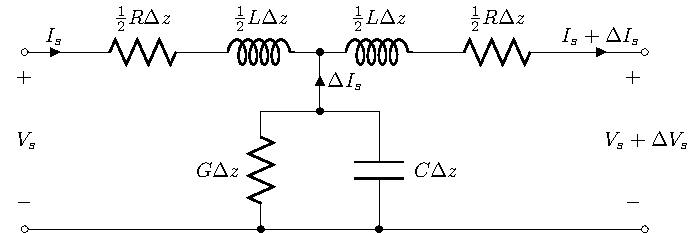
\includegraphics{figTransmissionBaicLines}
\caption{یکساں ترسیلی تار کا چھوٹا حصہ۔ متغیرات $R$، $L$، $C$ اور $G$ تار کی شکل اور مادوں پر منحصر ہیں۔}
\label{شکل_ترسیل_سادہ_نظام}
\end{figure}

یہاں بھی ہم موج کی حرکت \عددیء{\az} جانب تصور کرتے ہیں۔یوں تار کے چھوٹی لمبائی \عددیء{\Delta z} کی مزاحمت \عددیء{R \Delta z}، امالہ \عددیء{L \Delta z}، کپیسٹنس \عددیء{C \Delta z} اور ایصالیت \عددیء{G \Delta z} ہوں گے۔شکل \حوالہ{شکل_ترسیل_سادہ_نظام} میں ترسیلی تار کے اس چھوٹے لمبائی کو دکھایا گیا ہے۔چونکہ تار کا یہ چھوٹا ٹکڑا دونوں اطراف سے بالکل ایک جیسے معلوم ہوتا ہے  لہٰذا اس کے سلسلہ وار اجزاء کو آدھے آدھے ٹکڑوں میں کرتے ہوئے متوازی اجزاء کے دونوں طرف دکھایا گیا ہے۔ہم متوازی اجزاء کو دو برابر ٹکڑون میں کرتے ہوئے سلسلہ وار اجزاء کے دونوں جانب بھی جوڑ سکتے تھے۔

ہم فرض کرتے ہیں کہ شکل \حوالہ{شکل_ترسیل_سادہ_نظام} میں بائیں طرف برقی دباو
\begin{align*}
V=V_0 \cos (\omega t -\beta z +\psi)
\end{align*}
پائی جاتی ہے۔یہ حرکت کرتے موج کی عمومی مساوات ہے۔یولر\فرہنگ{یولر مماثل}\فرہنگ{Euler's identity} مماثل استعمال کرتے ہوئے اس مساوات کو
\begin{align*}
V=\left[ V_0 e^{j(\omega t -\beta z +\psi)}\right]_{\text{حقیقی}}
\end{align*}
لکھا جا سکتا ہے۔اس مساوات میں \عددیء{e^{j\omega t}} اور زیر نوشت میں \عددیء{_\text{حقیق}} کو پوشیدہ رکھتے ہوئے دوری سمتیہ کی صورت میں یوں لکھا جا سکتا ہے
\begin{align*}
V_s =V_0 e^{j \psi} e^{-\beta z}
\end{align*}
جہاں مساوات کے بائیں ہاتھ \عددیء{V_s} لکھتے ہوئے زیرنوشت میں \عددیء{s} یاد دلاتی ہے کہ یہ مساوات دوری سمتیہ کی شکل میں ہے۔ 

شکل \حوالہ{شکل_ترسیل_سادہ_نظام} کے گرد گھومتے ہوئے کرچاف کے برقی دباو کے قانون سے
\begin{align*}
V_s=\left(\frac{R\Delta z}{2} + j \frac{\omega L \Delta z}{2}\right) I_s+\left(\frac{R\Delta z}{2} + j \frac{\omega L \Delta z}{2}\right) \left(I_s+\Delta I_s \right)+V_s+\Delta V_s
\end{align*}
یا
\begin{align*}
\frac{\Delta V_s}{\Delta z} =-\left(R+j\omega L \right) I_s-\frac{1}{2}\left(R+j\omega L \right)\Delta I_s
\end{align*}
لکھا جا سکتا ہے۔اگر \عددیء{\Delta z} کو صفر کے قریب تر کیا جائے تب \عددیء{\Delta I_s} بھی صفر کے قریب تر ہو گا۔یوں \عددیء{\Delta z \to 0 } کی صورت میں اس مساوات کے آخری جزو کو نظر انداز کیا جا سکتا ہے۔یوں اسے
\begin{align}\label{مساوات_ترسیل_دباو_تفرقی_مساوات}
\frac{\dif V_s}{\dif z}=-\left(R+j\omega L \right) I_s
\end{align}
لکھا جا سکتا ہے۔

متوازی اجزاء پر برقی دباو
\begin{align*}
V_s-\left(\frac{R \Delta z}{2}+j\frac{\omega L \Delta z}{2} \right) I_s
\end{align*}
ہے جسے استعمال کرتے ہوئے شکل کو دیکھ کر متوازی اجزاء میں تفرقی رو کے لئے
\begin{align*}
-\Delta I_s = \left[V_s-\left(\frac{R \Delta z}{2}+j\frac{\omega L \Delta z}{2} \right) I_s \right] \left(G \Delta z+j \omega C \Delta z \right)
\end{align*}
یا
\begin{align*}
\frac{\Delta I_s}{\Delta z}=-\left(G+j \omega C \right) V_s +\frac{1}{2}\left(R+j \omega L \right)\left(G+j \omega C \right) I_s \Delta z
\end{align*}
لکھا جا سکتا ہے۔ اگر \عددیء{\Delta z \to 0} کیا جائے تب اس مساوات کے آخری جزو کو نظر انداز کیا جا سکتا ہے اور یوں
\begin{align}\label{مساوات_ترسیل_رو_تفرقی_مساوات}
\frac{\dif I_s}{\dif z}=-\left(G+j \omega C \right) V_s
\end{align}
 حاصل ہوتا ہے۔

یہاں رک کر ذرہ برقی و مقناطیسی امواج کے مساوات کو دوبارہ پیش کرتے ہیں۔میکس ویل کی مساوات
\begin{align*}
\nabla \times \kvec{E}_s=-j \omega \mu \kvec{H}_s
\end{align*}
میں \عددیء{\kvec{E}_s=E_{xs}\ax} اور \عددیء{\kvec{H}_{ys}=H_{ys}\ay}  پر کرنے سے
\begin{align}\label{مساوات_ترسیل_برقی_شدت_تفرقی_مساوات}
\frac{\dif E_{xs}}{\dif z}=-j \omega \mu H_{ys}
\end{align}
ملتا ہے اور اسی طرح
\begin{align*}
\nabla \times \kvec{H}_s=\left(\sigma+j\omega \epsilon \right)\kvec{E}_s
\end{align*}
سے
\begin{align}\label{مساوات_ترسیل_مقناطیسی_شدت_تفرقی_مساوات}
\frac{\dif H_{ys}}{\dif z}=-\left(\sigma+j \omega \epsilon \right) E_{xs}
\end{align}
ملتا ہے۔

مساوات \حوالہ{مساوات_ترسیل_رو_تفرقی_مساوات} کا مساوات \حوالہ{مساوات_ترسیل_مقناطیسی_شدت_تفرقی_مساوات} کے ساتھ موازنا کریں۔غور کرنے سے معلوم ہوتا ہے کہ پہلے مساوات میں \عددیء{I_s} کی جگہ \عددیء{H_{ys}} لکھنے اور اسی طرح \عددیء{G} کی جگہ \عددیء{\sigma}، \عددیء{C} کی جگہ \عددیء{\epsilon} اور \عددیء{V_s} کی جگہ \عددیء{E_{xs}} لکھتے ہوئے دوسری مساوات حاصل کی جا سکتی ہے۔دونوں مساوات بہت قریبی مشابہت رکھتے ہیں۔

اسی طرح مساوات \حوالہ{مساوات_ترسیل_دباو_تفرقی_مساوات} اور مساوات \حوالہ{مساوات_ترسیل_برقی_شدت_تفرقی_مساوات} کو دیکھتے ہوئے  یہی جوڑے یہاں بھی پائے جاتے ہیں، البتہ یہاں \عددیء{L} اور \عددیء{\mu} کی جوڑی بھی پائی جاتی ہے۔ہاں ظاہری طور پر \عددیء{R} کی جوڑی موجود نہیں ہے۔یوں ہم \عددیء{j \omega \mu} کی جوڑی \عددیء{R+j\omega L} لے سکتے ہیں۔

لامحدود یکساں مستوی امواج اور لامحدود لمبائی کی یکساں ترسیلی تار کے سرحدی شرائط ایک جیسے ہیں۔دونوں میں سرحد پایا ہی نہیں جاتا لہٰذا  ہم گزشتہ باب میں حاصل حل
\begin{align*}
E_{xs}=E_{x0} e^{- \gamma z}
\end{align*}
کی طرز پر اب
\begin{align}
V_s=V_0 e^{- \gamma z}
\end{align}
بطور ترسیلی تار کے مساوات کا حل لکھ سکتے ہیں۔یہ برقی دباو کے موج\فرہنگ{موج!برقی دباو}\فرہنگ{wave!voltage} کی مساوات ہے۔یہ موج مثبت \عددیء{z} جانب حرکت کر رہی ہے اور \عددیء{z=0} پر اس کا حیطہ \عددیء{V_0} ہے۔حرکی مستقل\فرہنگ{حرکی مستقل}\فرہنگ{propagation constant}
\begin{align*}
\gamma=\sqrt{j \omega \mu (\sigma +j\omega \epsilon)}
\end{align*}
اب
\begin{align}
\gamma=\alpha+j\beta=\sqrt{(R+j\omega L)(G+j\omega C)}
\end{align}
ہو جائے گا۔طول موج\فرہنگ{طول موج}\فرہنگ{موج!طول}\فرہنگ{wavelength} اب بھی
\begin{align}
\lambda=\frac{2\pi}{\beta}
\end{align}
ہو گا۔موج کی رفتار\فرہنگ{موج!رفتار}\فرہنگ{رفتار!موج}\فرہنگ{phase velocity} اب بھی
\begin{align}
v=\frac{\omega}{\beta}
\end{align}
ہے۔

کامل ترسیلی تار طاقت ضائع نہیں کرتا۔ایسی تار کے مستقل \عددیء{R=G=0} ہوتے ہیں لہٰذا
\begin{align*}
\gamma=j \beta=j \omega \sqrt{LC}
\end{align*}
اور 
\begin{align}
v=\frac{1}{\sqrt{LC}}
\end{align}
ہوں گے۔

اسی طرح مقناطیسی موج
\begin{align*}
H_{ys}=\frac{E_{x0}}{\eta} e^{-\gamma z}
\end{align*}
سے
\begin{align}
I_s=\frac{V_0}{Z_0} e^{-\gamma z}
\end{align}
لکھا جا سکتا ہے جہاں ترسیلی تار کی قدرتی رکاوٹ\فرہنگ{قدرتی رکاوٹ}\فرہنگ{intrinsic impedance} \عددیء{Z_0} کو
\begin{align*}
\eta=\sqrt{\frac{j\omega \mu}{\sigma +j\omega \epsilon}}
\end{align*}
سے
\begin{align}
Z_0=\sqrt{\frac{R+j\omega L}{G+j \omega C}}
\end{align}
لکھا جا سکتا ہے۔

خطہ-1 میں آمدی موج جب خطہ-2 کے سرحد سے ٹکراتی ہے تو اس کا کچھ حصہ بطور انعکاسی موج خطہ-1 میں واپس ہو جاتی ہے۔اس انعکاسی موج اور آمدی موج کی شرح کو شرح انعکاس\فرہنگ{شرح!انعکاس}\فرہنگ{reflection coefficient}
\begin{align*}
\Gamma=\frac{E_{x0}^-}{E_{x0}^+}=\frac{\eta_2-\eta_1}{\eta_2+\eta_1}
\end{align*}
کہتے ہیں۔اسی طرح اگر \عددیء{Z_{01}} قدرتی رکاوٹ کی ترسیلی تار پر آمد موج \عددیء{Z_{02}} قدرتی رکاوٹ کی ترسیلی تار میں داخل ہونا چاہے تو ان کے سرحد سے انعکاسی موج واپس ہو گی۔ایسی انعکاسی موج اور آمدی موج کی شرح
\begin{align}
\Gamma=\frac{V_0^-}{V_0^+}=\frac{Z_{02}-Z_{01}}{Z_{02}+Z_{01}}
\end{align}
 ہو گی۔انعکاسی شرح جانتے ہوئے شرح ساکن موج\فرہنگ{شرح!ساکن موج}\فرہنگ{standing wave ratio}
\begin{align}
s=\frac{1+\abs{\Gamma}}{1-\abs{\Gamma}}
\end{align}
لکھی جا سکتی ہے۔آخر میں اگر \عددیء{z>0} پر \عددیء{\eta=\eta_2} ہو تب \عددیء{z=-l} پر \عددیء{E_{xs}} اور \عددیء{H_{ys}} کی شرح 
\begin{align*}
\eta_{\text{داخلی}}=\eta_1 \frac{\eta_2+j \eta_1 \tan \beta_1 l}{\eta_1 +j \eta_2 \tan \beta_1 l}
\end{align*}
کو داخلی قدرتی رکاوٹ  کہتے ہیں۔اس سے \عددیء{z>0} پر \عددیء{Z_{02}} کی صورت میں ترسیلی تار کے لئے \عددیء{z=-l} پر \عددیء{V_s} اور \عددیء{I_s} کی شرح، یعنی اس کی داخلی قدرتی رکاوٹ\فرہنگ{داخلی قدرتی رکاوٹ}\فرہنگ{رکاوٹ!داخلی قدرتی}\فرہنگ{input intrinsic impedance} کو
\begin{align}
Z_{\text{داخلی}}=Z_{01} \frac{Z_{02}+j Z_{01}\tan \beta_1 l}{Z_{01}+j Z_{02}\tan \beta_1 l}
\end{align}
لکھا جا سکتا ہے۔
